\documentclass[conference]{IEEEtran}
\IEEEoverridecommandlockouts
% The preceding line is only needed to identify funding in the first footnote. If that is unneeded, please comment it out.
\usepackage{cite}
\usepackage{amsmath,amssymb,amsfonts}
\usepackage{algorithmic}
\usepackage{graphicx}
\usepackage{textcomp}
\usepackage{xcolor}
\usepackage{multicol}  
\usepackage{multirow}
\usepackage{booktabs} 
\usepackage{threeparttable}
\usepackage{algorithmic,algorithm}
\usepackage{subfigure}
%\usepackage{authblk}

\renewcommand{\algorithmicrequire}{ \textbf{Input:}} %Use Input in the format of Algorithm
\renewcommand{\algorithmicensure}{ \textbf{Output:}} %UseOutput in the format of Algorithm
\def\BibTeX{{\rm B\kern-.05em{\sc i\kern-.025em b}\kern-.08em
    T\kern-.1667em\lower.7ex\hbox{E}\kern-.125emX}}
\begin{document}

%\title{An Unbalanced Data Set Solution Based on FlowCGAN\\
\title{FlowCGAN: Exploratory Study of Class Imbalance for Encrypted Traffic Classification Using CGAN \\
%{\footnotesize 
%\textsuperscript{*}Note: Sub-titles are not captured in Xplore and
%should not be used}
%\thanks{Identify applicable funding agency here. If none, delete this.}
}

\author{\IEEEauthorblockN{1\textsuperscript{st} Shuhang Li}
\IEEEauthorblockA{\textit{School of Modern Posts} \\
\textit{Nanjing University}\\
\textit{of Posts\&Telecommunications}\\
Nanjing, China \\
lish@runtrend.com.cn}
\and
\IEEEauthorblockN{2\textsuperscript{nd} Pan Wang}
\IEEEauthorblockA{\textit{School of Modern Posts} \\
\textit{University of Nanjing University}\\
\textit{of Posts and Telecommunications}\\
Nanjing, China \\
wangpan@njupt.edu.cn}
\and
\IEEEauthorblockN{3\textsuperscript{rd} Xiaokang Zhou}
\IEEEauthorblockA{\textit{Faculty of Data Science } \\
\textit{Shiga University Hikone, Japan}\\
\textit{RIKEN Center for Advanced }\\
\textit{Intelligence Project}\\
Tokyo, Japan 
}
\and
\IEEEauthorblockN{4\textsuperscript{th} ZiXuan Wang}
\IEEEauthorblockA{\textit{School of Modern Posts} \\
\textit{University of Nanjing University}\\
\textit{of Posts and Telecommunications}\\
Nanjing, China \\
wangzx@runtrend.com.cn}
\and
\IEEEauthorblockN{5\textsuperscript{th} MoXuan Zhang}
\IEEEauthorblockA{\textit{Schools of International Education} \\
\textit{Jinling Institute of Technology}\\
Nanjing, China \\
zhangmoxuan\_7@126.com}
}


%\author{ShuHang Li$^{1}$ , Pan Wang $^{2}$ , Xiaokang Zhou $^{3}$ , ZiXuan Wang $^{1}$ ,MoXuan Zhang $^{4}$
%   \and
%   $^{1}$ School of Modern Posts, University of Nanjing University \\ of Posts and Telecommunications, Nanjing, China
%   \and
%   $^{2}$ YTO Express Co., Ltd., Shanghai,CO 201705,China
%   \and
%    Corresponding author: Pan Wang (e-mail: wangpan@njupt.edu.cn)
%}
%\author[1]{ShuHang Li}
%\author[1]{Pan Wang\thanks{Corresponding author: wangpan@njupt.edu.cn}}
%\author[2]{Xiaokang Zhou}
%\author[1]{ZiXuan Wang}
%\author[3]{MoXuan Zhang}
%\affil[1]{School of IOT,University of Nanjing University of Posts and Telecommunications}
%\affil[2]{Faculty of Data Science Shiga University Hikone, Japan,\authorcr RIKEN Center for Advanced Intelligence Project}
%\affil[3]{Schools of International Education,Jinling Institute of Technology}

\maketitle

\begin{abstract}
In the field of encrypted traffic identification, more and more researchers have begun to apply machine learning (ML), especially deep learning (DL) to traffic classification problems. Although these methods can automatically extract traffic features to overcome the difficulty of traditional classification methods like DPI in terms of feature engineering, a large amount of data is needed to learn the characteristics of various types of traffic. Therefore, the performance of classification model always significantly depends on the quality of the data set. The establishment of data sets is a time-consuming and laborious task. At the same time, it is often difficult to collect a large amount of traffic for some unpopular applications while traffic of hot applications is easy to access, which leads to the problem of data imbalances in data sets. In this paper, we proposed an unbalanced dataset solution based on FlowCGAN. As an instance of Generative Adversarial Nets(GAN), the method utilizes the advantage of GAN in data augmentation and generates new data samples by learning the characteristics of the traffic data, thereby achieving the purpose of balancing the data set. To verify the feasibility of this method, we use a classical deep learning model Convolutional Neural Networks(CNN) to classify the unbalanced data set, the random oversampled balanced data set, and the FlowCGAN balanced data set respectively. The experimental results show that the FlowCGAN method has better performance when compared with the other two data sets under the same conditions.
\end{abstract}

\begin{IEEEkeywords}
encrypted traffic identification, deep learning, Conditional Generative Adversarial Nets, traffic classification, data balance, convolutional neural network
\end{IEEEkeywords}

\section{Introduction}
With the rapid development of network technology, the types and quantity of traffic data in cyberspace are increasing. The identification and classification of network traffic is an important research content in the field of network management and network security. The ISP needs to perform dynamic access control according to the proportion of various types of traffic in the bandwidth to provide a better user experience for the customer. Security regulators need to detect malicious traffic in network traffic in real-time to avoid serious losses. As user privacy awareness increases and various encryption technologies mature, many Internet applications begin to encrypt their traffic data. At the same time, with the rapid development of 5G and the Internet of Things and the Industrial Internet, the node interaction information has high-security requirements, and the proportion of encrypted traffic in the network is also increasing. The emergence of encrypted traffic poses a huge challenge to the fields of network security, QoS, and network resource scheduling.

Traditional traffic identification technologies include the following: port-based matching~\cite{r1}, payload-based~\cite{r2}, and flow feature statistics. The emergence of various proprietary protocols and VPN tunneling technologies has made port matching technology quickly ineffective. To ensure the security of the data, the payload of the encrypted traffic is invisible, so the method based on the payload cannot cope with the classification problem of the encrypted traffic. To solve the above problems, researchers began to try to combine machine learning algorithms with flow statistics or timing features for traffic identification and classification~\cite{r3,r4,r5,r6}. However, this method has certain defects: (1) it is easy to be limited by the sample size, and it falls into the local optimal solution, and the generalization ability is poor; (2) the classification effect is greatly affected by the feature design, which brings uncertainty to the classification effect; (3) The lack of ability to automatically learn traffic characteristics requires manual design of features, resulting in models outdated rapidly. The emergence of deep learning has solved the above problems well. Some scholars use deep learning models such as CNN, MLP, SAE, LSTM, etc. to perform automatic feature extraction without human intervention~\cite{r7,r8,r9,r10}. The experimental results show that these methods are superior to traditional methods.

However, a large amount of data for feature learning is inseparable whether it is machine learning or deep learning. Due to the different heats of various applications, sample imbalances often occur when creating data sets. That is, the number of popular application samples is much larger than that of non-hot applications. During model training, the characteristics of small sample flows are easily masked by large samples, resulting in classification errors.

In this paper, we proposed an unbalanced dataset solution based on FlowCGAN, which utilizes the advantage of GAN in data augmentation, and generates a certain amount of minor class through feature learning to achieve the purpose of balancing the traffic data set. In this paper, the classical deep learning model CNN was used to classify the unbalanced data set, the random oversampled data set and the CGAN balanced data set to verify the feasibility of FlowCGAN data generation.

The subsequent chapters of this paper are organized as follows: Section~\ref{rw} describes the related works about solving the unbalanced data set; Section~\ref{gan} briefly describes the principles and network architecture of GAN and CGAN; Section~\ref{algorithm} elaborates on the methodology of FlowGAN, including data preprocessing, model architecture, and related algorithms; Section~\ref{results} describes the experimental environment and experimental results; Section~\ref{cof} provides conclusions about our work and an introduction to the future work.
\section{Related works}\label{rw}

%\subsection{Maintaining the Integrity of the Specifications}

In machine learning, scholars have done a lot of research on how to deal with unbalanced data sets~\cite{r14,r15,r16}. The most common methods for dealing with unbalanced data are: collect more traffic data, modifying objective cost functions, resampling and generating artificial data~\cite{r13}. The easiest way is to collect more small sample data, but this method often requires a lot of time, and the traffic data of some unpopular applications is difficult to collect. The main idea of modifying the objective cost function is to modify the sample weights, including increasing the weight of small samples and reducing the weight of large samples~\cite{r17}. The difficulty of this approach is how to determine the weight of each sample properly. Resampling includes two methods: random oversampling and random undersampling~\cite{r19}. Random undersampling randomly culling of some of the data in major class, while random oversampling randomly copying some data from the minor class to achieve the purpose of expanding the sample. However, this method does not generate new features in nature, it is only an extension of the number of minor class. The classic method of generating artificial data is the smote oversampling method, which constructs new sample data by randomly sampling the attribute values, not just the copying of the samples~\cite{r20}. However, it is possible to generate data that does not exist in reality and thereby destroy the linear relationship of the original features.

\section{Generative Adversarial Nets}\label{gan}

\subsection{GAN}\label{AA}

%Before you begin to format your paper, first write and save the content as a 
%separate text file. Complete all content and organizational editing before 
%formatting. Please note sections \ref{AA}--\ref{SCM} below for more information on 
%proofreading, spelling and grammar.

A classic GAN network consists of two parts, the generator $G$ and the discriminator $D$.GAN is unsupervised learning. The role of the generator is to simulate noise into real data by learning the characteristic distribution of real data. The discriminator aims at determining whether the sample is real data or data generated by $G$. 
%The basic framework of GAN is shown in Fig.~\ref{fig_gan}. 
The generator $G$ simulates the feature distribution $P_g$ of the real data by the prior distribution $P_z(z)$. The input of the discriminator is the real data and the generated data, and the output $D(x;\theta_d)$ indicates the probability of whether the sample data inputted  is real~\cite{r11}. During the training process, $G$ and $D$ play a mini-max game until $D$ can't judge whether the sample data is real, which means that the two networks reach the Nash balance. The objective function of GAN can be expressed by \eqref{GAN}:
\begin{equation}
\begin{split}
\label{GAN}
	\mathop {\min }\limits_{\rm{G}} \mathop {\max }\limits_D V(D,G) = \mathbb{E}_{x\sim{p_{data}}(x)}[\log D(x)] \\
+ {\mathbb{E}_{z\sim{p_z}(z)}}[\log (1 - D(G(z)))]
\end{split}
\end{equation}

\iffalse
\begin{figure}[htbp]
\centerline{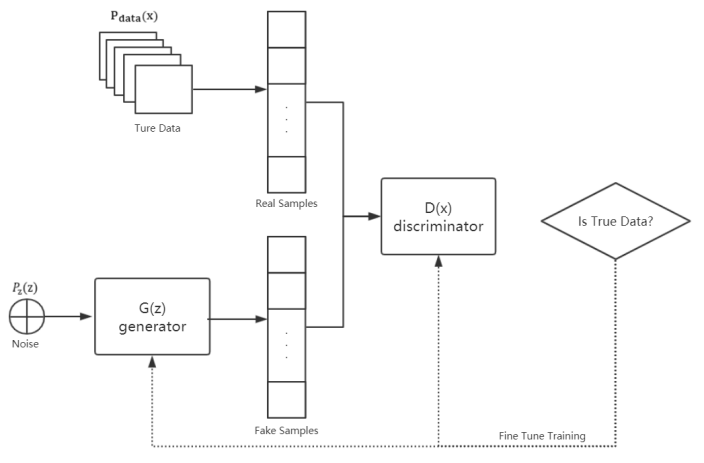
\includegraphics{fig/GAN.png}}
\caption{Network structure of GAN.}
\label{fig_gan}
\end{figure}
\fi 

In \eqref{GAN}, $P_{data}(x)$ represents the true data distribution. When training $D$, the goal is to judge $G(z)$ as the true probability $D(G(z))$ as small as possible and to judge the true data $x$ as the true probability $D\left(x\right)$ as large as possible. When training $G$, the goal is to make $D(G(z))$ as large as possible. From \eqref{GAN}, we can calculate the optimal discriminator as \eqref{eq1}. As can be seen from \eqref{eq1} below, when $P_{data}\left(x\right)=P_z\left(z\right)$, it means that $D$ cannot Distinguish whether the sample is true or false, $D$ and $G$ reach the Nash equilibrium, and the discriminator output is 0.5.

\begin{equation}
\begin{split}
\label{eq1}
	D^*(x)=\frac{P_{data}(x)}{P_{data}(x)+P_z(z)}
\end{split}
\end{equation}

\subsection{CGAN}

When compared with other complex generation models, GAN's game competition makes it possible to generate data without pre-modeling. It only needs to sample the distribution to approximate the real data. This is the biggest feature of GAN. This approach also has the disadvantage that it is too free and the output of the generator cannot be controlled by humans. For example, when training the Mnist dataset, the number output by the generator may be any number from 0-9. In order to solve this problem, Montreal proposed Conditional Generative Adversarial Nets CGAN~\cite{r12}. The method guides the data generation process by adding a constraint condition y to both $D$ and $G$. This simple improvement has proven to be very effective and widely used. Fig.~\ref{fig_cgan} shows the network structure of CGAN.

\begin{figure}[htbp]
\centerline{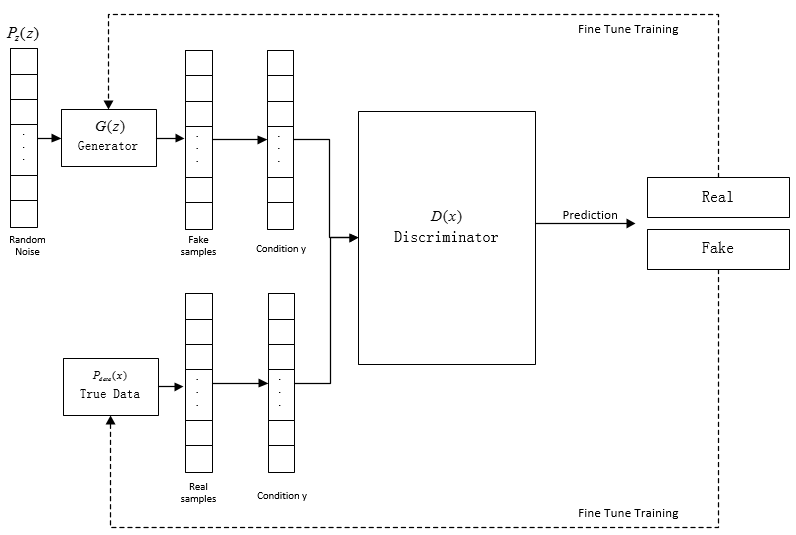
\includegraphics[width=8cm, height=6cm]{fig/cgan.png}}
\caption{The network structure of CGAN.}
\label{fig_cgan}
\end{figure}

The principle, structure and training process of CGAN are similar to GAN. The objective function is slightly different as is shown in \eqref{CGAN}:

\begin{equation}
\begin{split}
\label{CGAN}
	\mathop {\min }\limits_{\rm{G}} \mathop {\max }\limits_D V(D,G) = \mathbb{E}_{x\sim{p_{data}}(x)}[\log D(x|y)] \\
+ {\mathbb{E}_{z\sim{p_z}(z)}}[\log (1 - D(G(z|y)))]
\end{split}
\end{equation}

As shown in Fig.~\ref{fig_cgan}, CGAN's training process includes the following steps:
\begin{itemize}
\item Sampling the real data to obtain $P_{data}(x)$, obtaining the label y corresponding to the sampling data $P_{data}(x)$, feed $P_{data}(x)$ and y into the discriminator, and updating the parameters according to the output result;
\item Generate random noise $P_z(z)$, which is fed into generator $G$ together with label $y$ in the above step, and $G$ generates analog data.
\item Feed the analog data and the label $y$ generated in the above step into the discriminator, and $G$ adjusts the parameter according to the output result of $D$.
\item Repeat the above steps until $G$ and $D$ reach the Nash equilibrium
\end{itemize}

\section{The methodology of FlowGAN}\label{algorithm}
\subsection{Data preprocessing}\label{data_preprocess}
The captured network traffic data is often saved in PCAP or PCAPNG format when framing the data set. As the PCAP file format specification shows that the byte information of the data traffic type is saved in hexadecimal. When converted to decimal, the hexadecimal ranges from 0 to 255, which corresponds to the pixel range of the single-channel grayscale image. Therefore, traffic classification can refer to many deep learning methods for image recognition. However, PCAP packets can not directly be used for model training and need to be pre-processed.

Data preprocessing consists of three steps: filtering, specification length, and normalization. Fig.~\ref{preprocesse} is a flow chart of data preprocessing, which is detailed as follows:
\begin{itemize}
\item Load the entire PCAP file. Filter the first 24 bytes of the file header. This part only contains file information and does not help with traffic classification.
\item While cycle through the group information the traffic, grouping information is first filtered. Since the network environment is not guaranteed to be pure during the process of capturing traffic, it is necessary to filter some useless data packets, such as APR and DHCP.
\item Specification the length of the filtered packets. In the deep learning process, the model converts the input into a matrix for calculation, which requires the length of the data input to be consistent. The length of collected packet information tends to be different in each group, so it is necessary to truncate the long packet and padding the short packet. The specified packet length used in this paper is 1480, and the processed packet forms a Packet Byte Matrix (PBM) as an input to the deep learning model~\cite{r8}.
\item Data normalized. Limiting the pre-processed data to the range [0,1] can improve the accuracy and convergence speed of the model.
\item Data marked. Marke up the traffic information according to the application classification after processing.
\end{itemize}


\subsection{Unbalanced data set processing}\label{unbalanced_process}
In this paper, two methods were used to process the unbalanced dataset. The first one is a random oversampling method. The principle of this method is to randomly sample minor class to supplement the sample size. As this method is simple, the new data is only a copy of the original data, which will lead to the model learning wrong features easily, and even the over-fitting phenomenon. The second method is to generate minor sample data using a FlowCGAN generator that reaches the Nash balance. The data generated in this way is very close to the real data, and new sample features are introduced. The data balancing process is shown in Fig.~\ref{unba}. It includes the following processes: reading the data set and sample tags obtained in Section 4.1 above and obtaining the number of different samples; The number of each application that we set to train the FlowCGAN is 10,000. For major class, 10000 data is randomly sampled, and 4000 data for the minor class; Load the trained FlowCGAN model to generate 6000 small sample data by G, and merge with the data in the previous step to get a balanced data set.



\subsection{Algorithm Description}\label{algorithm_escription}
In the FlowCGAN designed in this paper, both $G$ and $D$ have a three-layer structure including an input layer, an output layer, and a hidden layer, as is shown in Fig.~\ref{cgan_model} below. CGAN's training steps mainly include the following three steps:

\begin{figure}[htbp]
\centerline{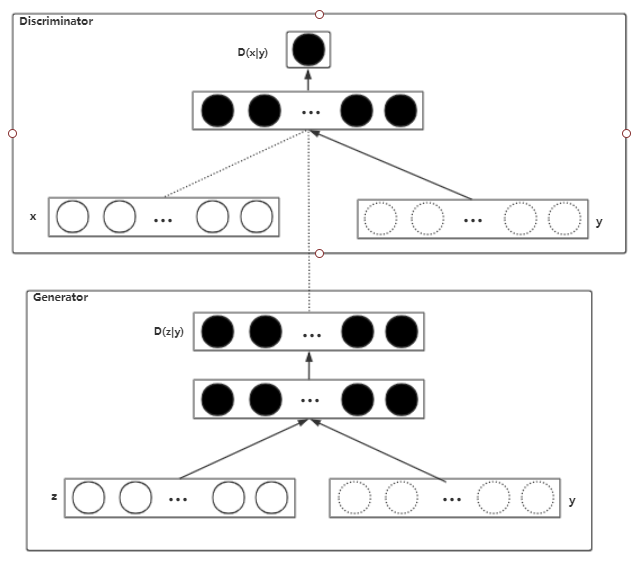
\includegraphics[width=8cm, height=8cm]{fig/cgan_model.png}}
\caption{The model architecture of CGAN.}
\label{cgan_model}
\end{figure}


Step one, train the discriminator. You need to fix the parameters of $G$ while training $D$. The data for the input layer is derived from the PBM packet byte matrix obtained in Section~\ref{data_preprocess} above, with a dimension of 1495. The hidden layer consists of 128 neurons, updating the weight of the input data and adding a bias:

\begin{equation}
\begin{split}
\label{d_input}
 D_{h1}=relu(input\cdot W_1+b_1)
\end{split}
\end{equation}

The 'input' in  \eqref{d_input} is composed of the real data $x$ and the sample label $y$. The hidden layer uses $ReLU$ as the activation function. The output layer has only one neuron, and the data from the hidden layer is weighted and offset to obtain the probability that if the sample is true:

\begin{equation}
\begin{split}
\label{d_output}
 d\_out=D_{h1}\cdot W_2+b_2
\end{split}
\end{equation}



\begin{figure*}[htbp]
\centering
\subfigure[Data Preprocessing]{
\begin{minipage}[t]{0.33\linewidth}
\centering
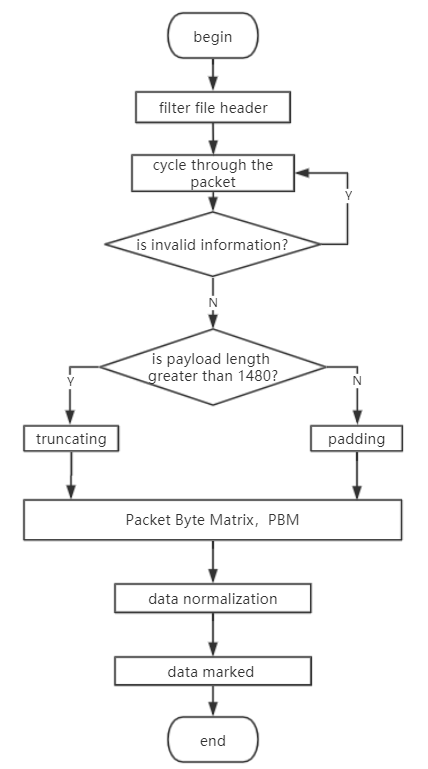
\includegraphics[width=1.6in]{fig/preprocesse.png}
\label{preprocesse}
\end{minipage}%
}%
\subfigure[FlowCGAN Model Training]{
\begin{minipage}[t]{0.33\linewidth}
\centering
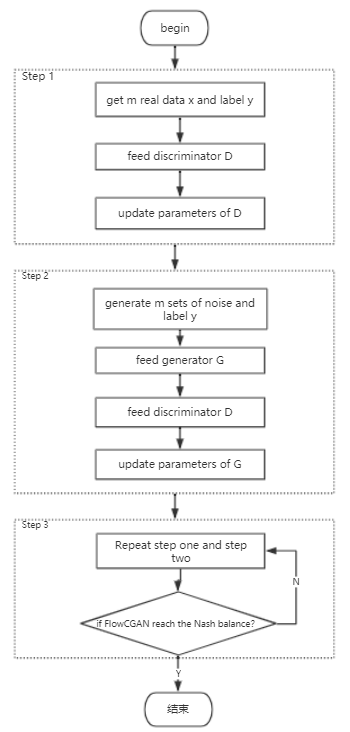
\includegraphics[width=1.6in]{fig/cgan_train.png}
\label{cgan_train}
\end{minipage}%
}%
\subfigure[Unbalanced Dataset Processing]{
\begin{minipage}[t]{0.33\linewidth}
\centering
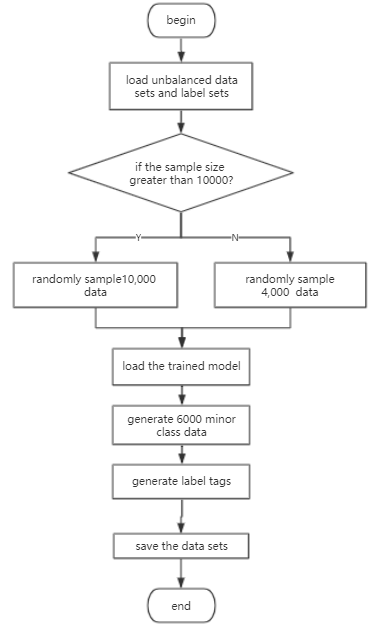
\includegraphics[width=1.6in]{fig/unba.png}
\label{unba}
\end{minipage}%
}%
\caption{The methodology of FlowGAN}
\label{methodology}
\end{figure*}


The model uses the Adam optimization algorithm as the optimizer to update weights $W_1$, $W_2$ and offsets $b_1$,  $b_2$. The overall training process of the discriminator is shown in Algorithm.~\ref{algorithm:discriminator}, in which $X_{\tau}=\begin{pmatrix}
x_{11}&\cdots&x_{1k}\\
\vdots&\ddots&\vdots\\
x_{m1}&\cdots&x_{mk}
\end{pmatrix}$
,$y_{\tau}=\begin{pmatrix}
y_{11}\\
\vdots\\
y_{m1}
\end{pmatrix}$
,k is identical to the value of data dimension:1480,$m$ equals to the value of mini\_batch.

\begin{algorithm}[htbp]
	\caption{Discriminator of FlowCGAN training}  \label{algorithm:discriminator}
	\begin{algorithmic}[1]  
		\REQUIRE real data $X_{\tau}$ and label $y_{\tau}$ from Section ~\ref{unbalanced_process},$\tau$ is the number of iterations
		\ENSURE Scores of the input data $d_{\tau}$
		\STATE Set the relevant initialization parameters,e represents the training cycle: epoches.
		\FOR {$\tau$ in $e$ }
		\FOR {each batch of $m$ input data}
		\STATE concat $X_\tau$ with $y_\tau$: 
		\STATE Compute the output using Equation.~(\ref{d_input});
		\STATE Compute the output using Equation.~(\ref{d_output});
		\STATE Output distinguishing results according to Equation.~(\ref{d_output});
		\STATE Optimal the loss function
		\STATE Update weights and bias;
		\ENDFOR \\ % end for mini_batch
		\ENDFOR \\ %end for epoch
	\end{algorithmic}  
\end{algorithm}  

Step two, train the generator $G$.The parameters of $D$ need to be fixed like step one. The input layer of $G$ consists of 115 neurons, and the input data includes stochastic noise $P_z(z)$ and sample label $y$. The hidden layer also has 128 neurons to update the weight and offset of the input data:

\begin{equation}
\begin{split}
\label{g_input}
 G_{h1}=relu(input\cdot W_1+b_1)
\end{split}
\end{equation}

The 'input' in \eqref{g_output} is made up of random noise $P_z(z)$ and the sample label $y$, and $ReLu$ is also used as the activation function. The output layer contains 1480 neurons, weighting and biasing the output of the hidden layer. The computed result will be activated by the sigmoid function.

\begin{equation}
\begin{split}
\label{g_output}
 g\_out=sigmoid(G_{h1}\cdot W_2+b_2)
\end{split}
\end{equation}

The optimization function is the same as the discriminator. The generator training algorithm is shown in Algorithm.~\ref{algorithm:generator}.The sample label $y$ in Algorithm.~\ref{algorithm:generator} should be consistent with $y$ in Algorithm.~\ref{algorithm:discriminator}.
$Z_{\tau}=\begin{pmatrix}
z_{11}&\cdots&z_{1n}\\
\vdots&\ddots&\vdots\\
z_{m1}&\cdots&z_{mn}
\end{pmatrix}$,$n=100$.

\begin{algorithm}[htbp]
	\caption{Generator of FlowCGAN training}  \label{algorithm:generator}
	\begin{algorithmic}[1]  
		\REQUIRE random noise $Z_{\tau}$, and label $y_{\tau}$,$\tau$ is the number of iterations
		\ENSURE generation data $g_{\tau}$
		\STATE Set the relevant initialization parameters,e represents the training cycle: epoches.
		\FOR {$\tau$ in $e$ }
		\FOR {each batch of $m$ input data}
		\STATE concat $Z_\tau$ with $y_\tau$: 
		\STATE Compute the output using Equation.~(\ref{g_input});
		\STATE Compute the output using Equation.~(\ref{g_output});
		\STATE Output generation data according to Equation.~(\ref{g_output});
		\STATE Optimal the loss function
		\STATE Update weights and bias;
		\ENDFOR \\ % end for mini_batch
		\ENDFOR \\ %end for epoch
	\end{algorithmic}  
\end{algorithm}  

\begin{figure}[htbp]
\centerline{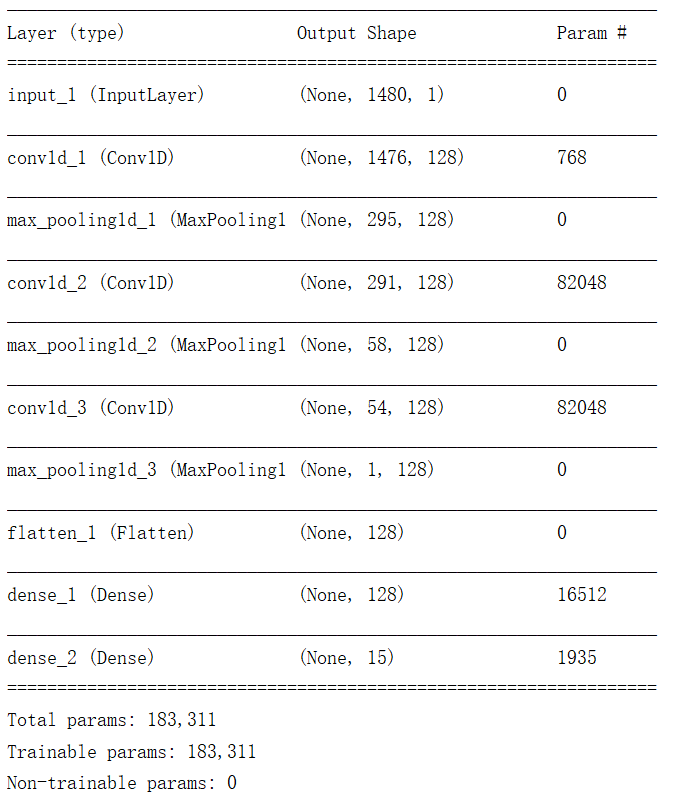
\includegraphics[width=8cm, height=8cm]{fig/cnn.png}}
\caption{Model architecture of CNN.}
\label{cnn}
\end{figure}

\section{Experimental result}\label{results}
\subsection {Experimental environmental}

The experimental environmental parameters of this paper are shown in Table~\ref{parameters}. To verify the feasibility of the FlowCGAN algorithm, we set up an unbalanced data set, a random oversampling balanced data set, and a FlowCGAN balanced data set for comparison. The classification of the three data sets was verified by the CNN convolutional neural network, the most basic deep learning model. As shown in Fig.~\ref{cnn}, we design a simple CNN model for encrypted traffic identification. The model uses 1 input layer, 1480 neurons; 3 convolution layers and pooling layer, composed of 128 convolution kernels, activated by ReLU; a fully connected layer of 128 neurons and an output layer, 15 neurons, and the activation function is Softmax for classification. Table~\ref{training_parameters} shows the parameters of the optimizer, loss function, epoches, and mini\_batch used in the deep training model training process.
%Table~\ref{tab:generator_desc} and Table~\ref{tab:discriminator_desc} describe the model architecture of  Generator and Discriminator in our experiments.


\linespread{1.5}
\begin{table}[htbp]
\caption{Experimental Environment Parameters}
\begin{center}
\begin{tabular}{c c}
\hline
\textbf{Category}&{\textbf{Parameters}} \\
\hline
%\cline{1-2} 
%\textbf{Head} & \textbf{\textit{Table column subhead}}& \textbf{\textit{Subhead}}& \textbf{\textit{Subhead}} \\
%\hline
GPU & Nvidia GPU(GeForce GTX 1660Ti)  \\
%\hline
Operating System & Win 10 \\
Deep learning platform & TensorFlow 1.13.1 + Keras 1.0.7\\
CUDA Version & 9.0\\
CuDNN Version & 7.6.0
\end{tabular}
\label{parameters}
\end{center}
\end{table}

\linespread{1.5}
\begin{table}[htbp]
\fontsize{6.5}{8}
\caption{Training Parameters}
\begin{center}
\begin{tabular}{c c c c}
\hline
\textbf{Training Parameters}&{\textbf{Generator}}&{\textbf{Discriminator}}&{\textbf{CNN}} \\
\hline
%\cline{1-2} 
%\textbf{Head} & \textbf{\textit{Table column subhead}}& \textbf{\textit{Subhead}}& \textbf{\textit{Subhead}} \\
%\hline
Optimizer & Adma & Adma & rmsprop  \\
%\hline
Loss Function & Cross-Entropy & Cross-Entropy &Cross-Entropy \\
Epoches & 200000 & 200000 & 50\\
Mini\_batch & 64 & 64 & 256\\

\end{tabular}
\label{training_parameters}
\end{center}
\end{table}



\subsection {Dataset for train}
The dataset for evaluation is selected from the "ISCX VPN\-nonVPN traffic dataset"~\cite{r21}. The dataset contains many encryption applications, protocols such as HTTPS, SFTP, Facebook, Hangouts, etc. A regular session and a session over VPN were captured in this dataset. 15 applications were chosen to make up the training samples for CGAN as Table~\ref{tab:Desc_Samples} shows. The majority classes such as NetFlix accounting for 25.13\% in the selected dataset, while the minimal sample size ICQ account for only 2.05\%. The number of traffic per application in the balanced data set is 10,000.

%\begin{table}[tp]  
\begin{table}[htbp]	
	\centering  
	\fontsize{6.5}{8}\selectfont  
	\begin{threeparttable}  
		\caption{Description of the chosen datasets.}  \label{tab:Desc_Samples}  
		\begin{tabular}{l|c|cc|cc|}  
			\toprule  
			\multirow{2}{*}{\textbf{Application}}&
			\multirow{2}{*}{\textbf{Security}}&
			\multicolumn{2}{c}{\textbf{Unbalanced dataset}}&\multicolumn{2}{|c}{\textbf{Balanced  dataset}} \cr  
			\cmidrule(lr){3-4} \cmidrule(lr){5-6}  
			&\textbf{Protocol} & \textbf{Quantity} & \textbf{Percentage} & \textbf{Quantity} & \textbf{Percentage}\cr  
			
			\midrule  
			AIM				&HTTPS	 	   &4869&2.356\%	  &10000&6.67\%\cr  
			Email-Client&SSL			  &4417&2.137\%		 &10000&6.67\%\cr  
			Facebook	&HTTPS	 	   &5527&2.674\%	  &10000&6.67\%\cr  
			Gmail		   &HTTPS		  &7329&3.546\%		 &10000&6.67\%\cr  
			Hangout		&HTTPS	 	   &7587&3.671\%	  &10000&6.67\%\cr  
			ICQ				&HTTPS	 	   &4243&2.053\%	  &10000&6.67\%\cr  
			Netflix			&HTTPS		   &51932&25.126\%	&10000&6.67\%\cr  
			SCP				&SSH	  		 &15390&7.446\%	   &10000&6.67\%\cr  
			SFTP			&SSH	 		 &4729&2.287\%	    &10000&6.67\%\cr  
			Skype		   &proprietary	 &4607&2.229\%	    &10000&6.67\%\cr  
			Spotify		   &proprietary	 &14442&6.987\%	   &10000&6.67\%\cr  
			torTwitter	  &proprietary	&14654&7.089\%	  &10000&6.67\%\cr  
			Vimeo		  &HTTPS		  &18755&9.074\%	&10000&6.67\%\cr  
			voipbuster	&proprietary   &35469&17.161\%	&10000&6.67\%\cr  
			Youtube		&HTTPS			 &12738&6.163\%	   &10000&6.67\%\cr  							
			\midrule
			
			TOTAL&  &{\bf 206688}&{\bf 100\%}&{\bf 150000}&{\bf 100\%}
		\end{tabular}  
	\end{threeparttable}  
\end{table}  

\subsection {Performance metrics}
In order to evaluate the performance of the model, we used the following three indicators: Precision, Recall, and F1-Score. FP(False Positive) means that the traffic of non-category C (C refers to a specific category) is classified into category C; TN(True Negative) means that streams of non-category C are classified into non-category C. FN(False Negative) means that traffic belonging to category C is classified as non-category C; TP(True Positive) refers to traffic belonging to category C and is classified into category C.F1-Score is the weighted harmonic average of the accuracy rate and the recall rate~\cite{r18}, which is used to comprehensively reflect the overall indicator.


\begin{itemize}
\item Precision:
	\begin{equation}
	\begin{split}
	\label{Precision}
 	Precision=\frac{TP}{TP+FN}
	\end{split}
	\end{equation}
\item Recall:
	\begin{equation}
	\begin{split}
	\label{Recall}
 	Recall=\frac{TP}{TP+FP}
	\end{split}
	\end{equation}
\item F1-Score:
	\begin{equation}
	\begin{split}
	\label{Recall}
 	F1-Score=\frac{2\cdot{Precision}\cdot{Recall}}{Precision+Recall}
	\end{split}
	\end{equation}

\end{itemize}

\subsection {Analysis of experimental results}
Figure~\ref{cgan_loss} shows the trend of loss of generator and discriminator during the FlowCGAN training process. It can be seen that CGAN does not change the instability characteristics of GAN. The loss of $G$ and $D$ always fluctuates within a range instead of reaching a convergence value.

Fig~\ref{matrices} shows the classification confusion matrices of three datasets based on the CNN-based encrypted traffic identification model, in which the elements on the diagonal representing the correct classification, and all other elements are misjudged. It can be clearly seen that the false positive rate of minor class in Fig~\ref{imBamatrices} is higher than Fig~\ref{osmatrices} and Fig~\ref{cganmatrices}.

Fig~\ref{performance} shows the performance indicators of the three data sets more clearly. As we can see from Fig~\ref{performance} that FlowCGAN performs best in the minor class except for ICQ. The performance metrics of ICQ in the unbalanced dataset were aways higher better than the two balanced datasets.

\begin{figure}[htbp]
\centering
\subfigure[d loss]{
\begin{minipage}[t]{0.5\linewidth}
\centering
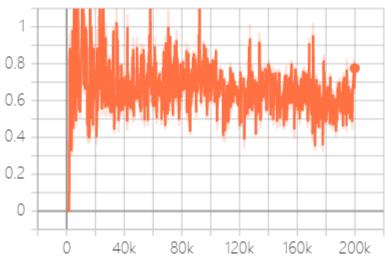
\includegraphics[width=1.6in]{fig/dloss.png}
\end{minipage}%
}%
\subfigure[g loss]{
\begin{minipage}[t]{0.5\linewidth}
\centering
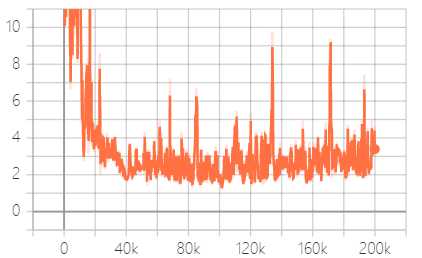
\includegraphics[width=1.7in]{fig/gloss.png}
\end{minipage}%
}%
\caption{Loss of FlowCGAN}
\label{cgan_loss}
\end{figure}

\begin{table}[htb]
	\centering
	\fontsize{6.5}{8}
	\caption{Performance of CNN-based traffic classifier.}\label{table:performance_classifier}
	\begin{tabular}{|l|c|c|c|c|}% left center and right.
		\hline
		data augmenting methods & Accuracy & Precision & Recall & F1-Score \\
		\hline
		\textbf{results of unbalanced dataset}  & 0.9897 & 0.9759 & 0.9775 &  0.9766 \\
		\hline
		\textbf{results of oversampling dataset}   & 0.9889 & 0.9892 & 0.9889& 0.989 \\
		\hline
		\textbf{results of CGAN dataset}   & 0.9951 & 0.9951 & 0.9951  & 0.9951 \\
		\hline
	\end{tabular}
\end{table}

\begin{figure*}[htb]
\centering
\subfigure[confusion matrix of unbalanced dataset]{
\begin{minipage}[t]{0.33\linewidth}
\centering
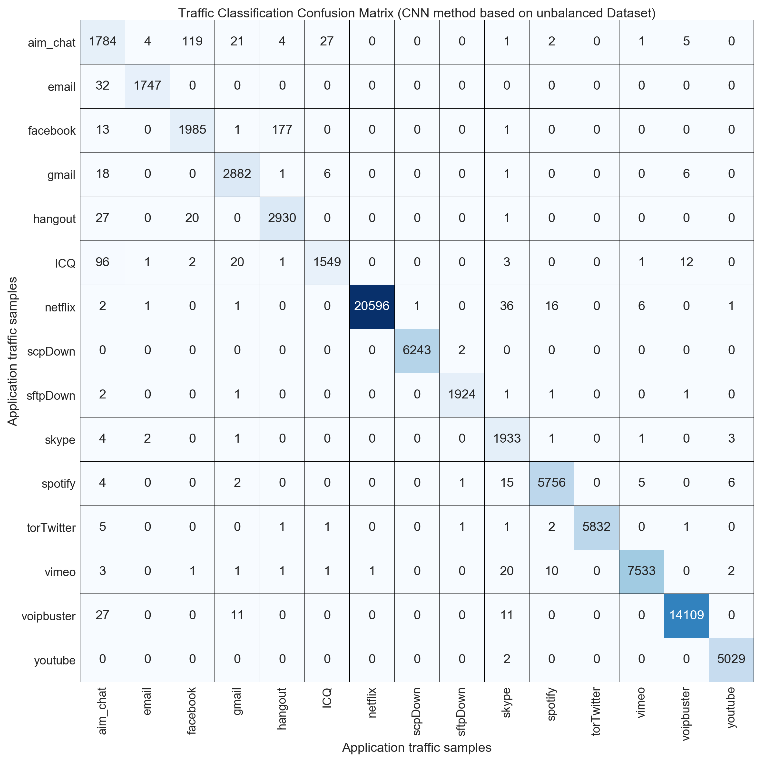
\includegraphics[width=2in]{fig/unba_h.png}
\label{imBamatrices}
\end{minipage}%
}%
\subfigure[confusion matrix of oversampling dataset]{
\begin{minipage}[t]{0.33\linewidth}
\centering
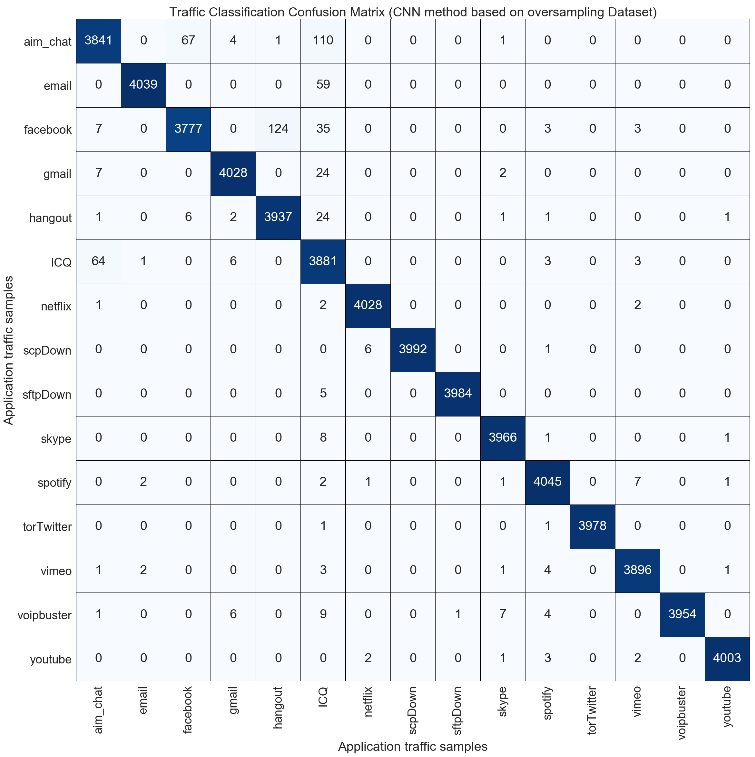
\includegraphics[width=2in]{fig/os_h.png}
\label{osmatrices}
\end{minipage}%
}%
\subfigure[confusion matrix of FlowCGAN dataset]{
\begin{minipage}[t]{0.33\linewidth}
\centering
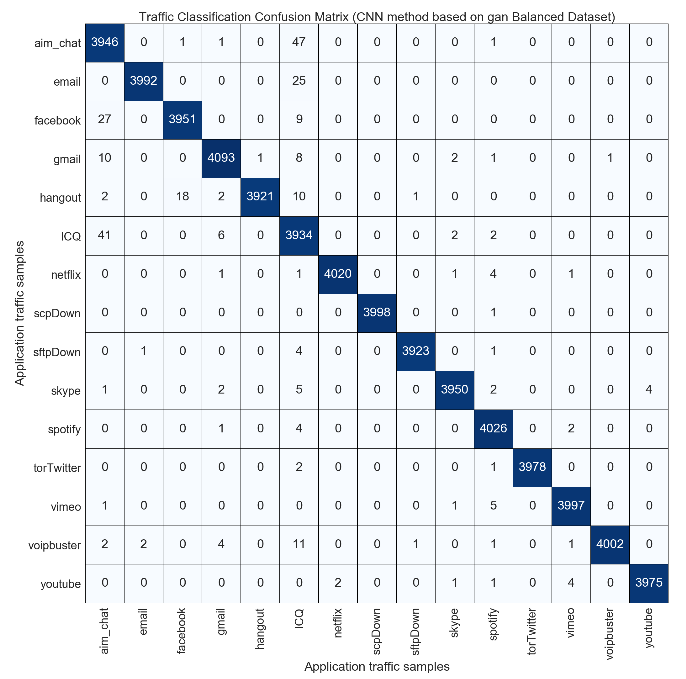
\includegraphics[width=2in]{fig/gan_h.png}
\label{cganmatrices}
\end{minipage}%
}%
\caption{Confusion matrices of CNN-based encrypted traffic identification method}
\label{matrices}
\end{figure*}

\begin{figure*}[htb]
\centering
\subfigure[performance metrics of the unbalanced dataset]{
\begin{minipage}[t]{0.33\linewidth}
\centering
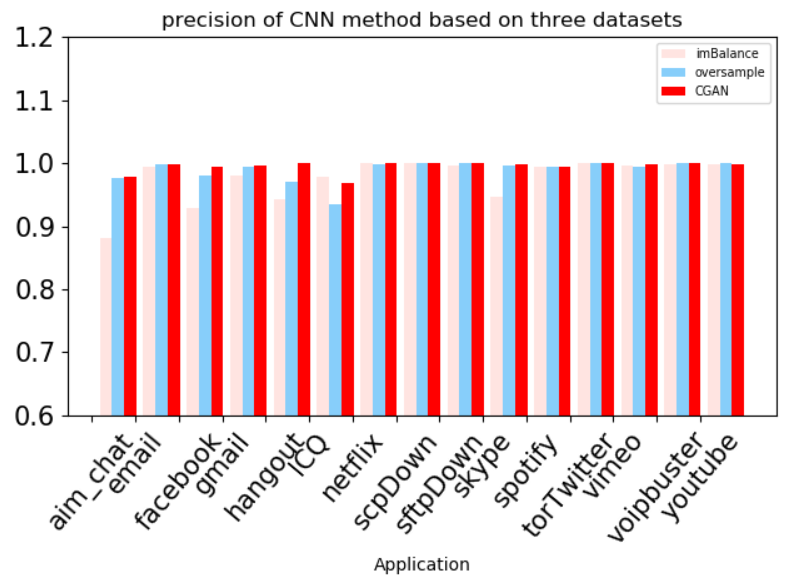
\includegraphics[width=2in]{fig/cnn_pre.png}
\end{minipage}%
}%
\subfigure[performance metrics of oversampling dataset]{
\begin{minipage}[t]{0.33\linewidth}
\centering
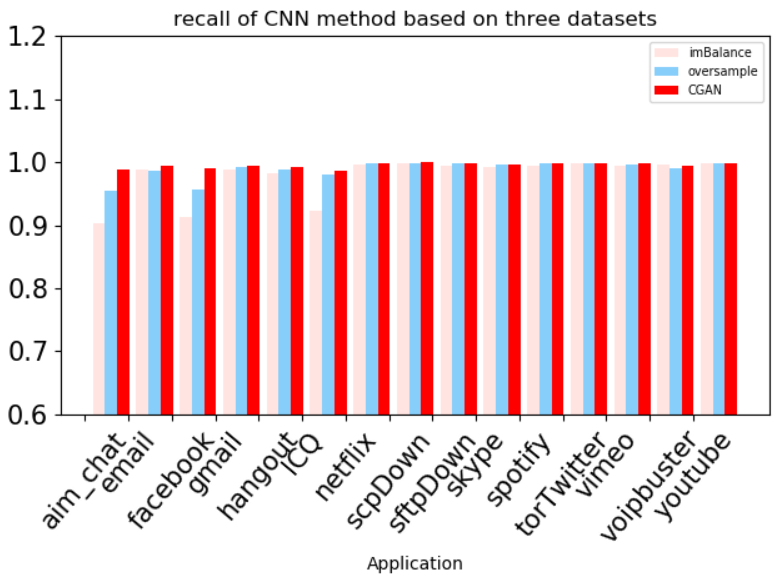
\includegraphics[width=2in]{fig/cnn_rec.png}
\end{minipage}%
}%
\subfigure[performance metrics of FlowCGAN dataset]{
\begin{minipage}[t]{0.33\linewidth}
\centering
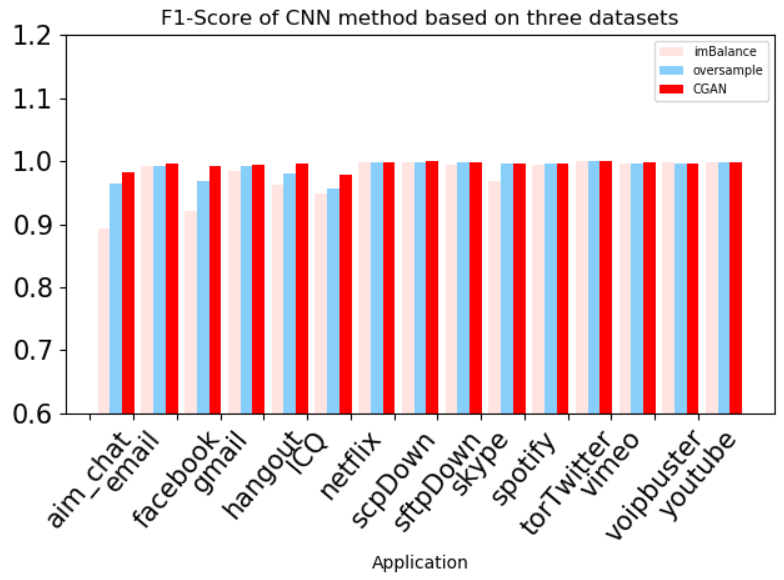
\includegraphics[width=2in]{fig/cnn_f1.png}
\end{minipage}%
}%
\caption{Performance metrics of CNN-based encrypted traffic identification method}
\label{performance}
\end{figure*}

\begin{table*}[htb]	
	\centering  
	\fontsize{6.5}{8}\selectfont  
	\begin{threeparttable}  
		\caption{Description of experimental results}  \label{tab:Desc_Samples}  
		\begin{tabular}{l|ccc|ccc|ccc|}  
			\toprule  
			\multirow{2}{*}{\textbf{Application}}&
			\multicolumn{3}{c}{\textbf{Unbalanced dataset}}&\multicolumn{3}{|c}{\textbf{oversampling Balanced  dataset}}&\multicolumn{3}{|c}{\textbf{CGAN Balanced  dataset}} \cr  
			\cmidrule(lr){2-4} \cmidrule(lr){5-7}  \cmidrule(lr){8-10} 
			&\textbf{Precision} & \textbf{Recall} & \textbf{F1-Score} &\textbf{Precision} & \textbf{Recall} & \textbf{F1-Score}&\textbf{Precision} & \textbf{Recall} & \textbf{F1-Score}\cr  
			
			\midrule  
				AIM			 & 0.8823&0.9027&0.8924  & 0.9757&0.9557&0.9656 &	0.9792&0.9875&0.9833 \cr
				Email-Client & 0.9949&0.9893&0.9921 & 0.9985&0.9866&0.9925 &	0.9992&0.9938&0.9965 \cr
				Facebook	 & 0.9287&0.913&0.9208 & 0.9808&0.9571&0.9688 &	0.9952&0.991&0.9931 \cr
				Gmail		 & 0.9803&0.988&0.9841 & 0.9939&0.9919&0.9929 &	0.9959&0.9944&0.9951 \cr
				Hangout		 & 0.9421&0.9827&0.962 & 0.9712&0.9881&0.9796 &	0.9997&0.9917&0.9957 \cr
				ICQ			 & 0.9778&0.9225&0.9494 & 0.9343&0.9807&0.9569 &	0.969&0.9872&0.978 \cr
				Netflix		 & 0.9999&0.9965&0.9982 & 0.9983&0.9978&0.998 &	0.9995&0.998&0.9988 \cr
				SCP			 & 0.9997&0.9989&0.9993 & 1&0.9982&0.9991 &	1&0.9997&0.9999 \cr
				SFTP		 & 0.9963&0.9942&0.9952 & 0.9995&0.998&0.9988 &	0.9995&0.9985&0.999 \cr
				Skype		 & 0.9473&0.992&0.9692 & 0.996&0.996&0.996 &	0.9982&0.9965&0.9973 \cr
				Spotify		 & 0.995&0.9935&0.9942 & 0.9952&0.9975&0.9964 &	0.9951&0.9983&0.9967 \cr
				torTwitter & 1&0.9993&0.9997 & 1&0.9992&0.9996 &	1&0.9992&0.9996 \cr
				Vimeo		 & 0.9973&0.9951&0.9962 & 0.9948&0.9973&0.9961 &	0.998&0.9983&0.9981 \cr
				voipbuster & 0.9991&0.9965&0.9978 & 1&0.9909&0.9954 &	0.9998&0.9945&0.9971 \cr
				Youtube		 & 0.9975&0.9986&0.998 & 0.9997&0.9982&0.999 &	0.999&0.998&0.9985 \cr						
			\midrule
			
			Average&{\bf 0.9759}&{\bf 0.9775}&{\bf 0.9766}&{\bf 0.9892}&{\bf 0.9889}&{\bf 0.989}&{\bf 0.9951}&{\bf 0.9951}&{\bf 0.9951}
		\end{tabular}  
	\end{threeparttable}  
\end{table*}  

\section{Conclusion and Future work}\label{cof}
In this paper, we proposed a CGAN-based traffic data enhancement method called FlowCGAN to solve the problem of unbalanced sample size in the dataset. After the specified sample data is generated by the generator, The generated data is combined with the original data to construct a new balanced dataset. We use CNN to verify the classification effect of different data sets. The experimental results show that the balanced data set generated by FlowCGAN has better performance. In the future, we will further study other types of GAN applications in traffic classification and  try to solve the problem of unstable training.

\section*{Acknowledgment}
This work was supported by the National Science Foundation of China (61972211)



\iffalse
\subsection{Figures and Tables}
\paragraph{Positioning Figures and Tables} Place figures and tables at the top and 
bottom of columns. Avoid placing them in the middle of columns. Large 
figures and tables may span across both columns. Figure captions should be 
below the figures; table heads should appear above the tables. Insert 
figures and tables after they are cited in the text. Use the abbreviation 
``Fig.~\ref{fig}'', even at the beginning of a sentence.

\begin{table}[htbp]
\caption{Table Type Styles}
\begin{center}
\begin{tabular}{|c|c|c|c|}
\hline
\textbf{Table}&\multicolumn{3}{|c|}{\textbf{Table Column Head}} \\
\cline{2-4} 
\textbf{Head} & \textbf{\textit{Table column subhead}}& \textbf{\textit{Subhead}}& \textbf{\textit{Subhead}} \\
\hline
copy& More table copy$^{\mathrm{a}}$& &  \\
\hline
\multicolumn{4}{l}{$^{\mathrm{a}}$Sample of a Table footnote.}
\end{tabular}
\label{tab1}
\end{center}
\end{table}

\begin{figure}[htbp]
\centerline{\includegraphics{fig/fig1.png}}
\caption{Example of a figure caption.}
\label{fig}
\end{figure}




Figure Labels: Use 8 point Times New Roman for Figure labels. Use words 
rather than symbols or abbreviations when writing Figure axis labels to 
avoid confusing the reader. As an example, write the quantity 
``Magnetization'', or ``Magnetization, M'', not just ``M''. If including 
units in the label, present them within parentheses. Do not label axes only 
with units. In the example, write ``Magnetization (A/m)'' or ``Magnetization 
\{A[m(1)]\}'', not just ``A/m''. Do not label axes with a ratio of 
quantities and units. For example, write ``Temperature (K)'', not 
``Temperature/K''.




\section*{Acknowledgment}

The preferred spelling of the word ``acknowledgment'' in America is without 
an ``e'' after the ``g''. Avoid the stilted expression ``one of us (R. B. 
G.) thanks $\ldots$''. Instead, try ``R. B. G. thanks$\ldots$''. Put sponsor 
acknowledgments in the unnumbered footnote on the first page.

\section*{References}

Please number citations consecutively within brackets \cite{b1}. The 
sentence punctuation follows the bracket \cite{b2}. Refer simply to the reference 
number, as in \cite{b3}---do not use ``Ref. \cite{b3}'' or ``reference \cite{b3}'' except at 
the beginning of a sentence: ``Reference \cite{b3} was the first $\ldots$''

Number footnotes separately in superscripts. Place the actual footnote at 
the bottom of the column in which it was cited. Do not put footnotes in the 
abstract or reference list. Use letters for table footnotes.

Unless there are six authors or more give all authors' names; do not use 
``et al.''. Papers that have not been published, even if they have been 
submitted for publication, should be cited as ``unpublished'' \cite{b4}. Papers 
that have been accepted for publication should be cited as ``in press'' \cite{b5}. 
Capitalize only the first word in a paper title, except for proper nouns and 
element symbols.

For papers published in translation journals, please give the English 
citation first, followed by the original foreign-language citation \cite{b6}.

\begin{thebibliography}{00}

\bibitem{r15} C. Chen, A. Liaw, and L. Breiman. Using random forest to learn imbalanced data. In Technical report, 2013.
\bibitem{r16} H. M. Nguyen, E. W. Cooper, and K. Kamei.Borderline over-sampling for imbalanced data. In Fifth International Workshop on Computational Intelligence and Applications IEEE, 2009.
\bibitem{r17} L. Cao, J. Zhong, and Y. Feng. Cost sensitive classification in data mining. In LNCS 6440 Part I,2010.
\end{thebibliography}
\fi

\vspace{12pt}

\bibliographystyle{IEEEtran}      %IEEEtran为给定模板格式定义文件名

\bibliography{Reference}                        %ref为.bib文件名

%{\bf\normalsize Biography}
%
%\begin{figure}[ht!]
%	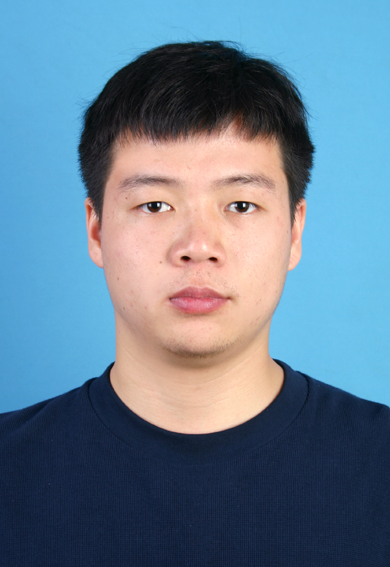
\includegraphics[width=1 in]{fig/li} 
%\end{figure}
%\noindent{\it ShuHang Li} was graduated from Jiangsu University of Science and Technology,Zhenjiang ,China, in 2013.He is currently pursuing a master's degree at Nanjing University of Posts \& Telecommunications,Nanjing China.His research direction is encrypted traffic identification,and he also interested in Deep Packet Inspection and applications.(email:lish@runtrend.com.cn)
%
%\begin{figure}[ht!]
%	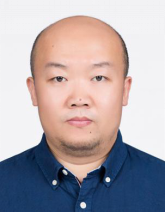
\includegraphics[width=1 in]{fig/wp} 
%\end{figure}
%
%\noindent{\it Pan Wang} (M'18) received the BS degree from the Department of Communication Engineering, Nanjing University of Posts \& Telecommunications, Nanjing, China, in 2001, and the PhD degree in Electrical \& Computer Engineering from Nanjing University of Posts \& Telecommunications, Nanjing, China, in 2013. He is currently an Associate Professor in the School of Modern Posts, Nanjing University of Posts \& Telecommunications, Nanjing, China. His research interests include cyber security and communication network security, network measurements, Quality of Service, Deep Packet Inspection, SDN, big data analytics and applications. From 2017 to 2018, he was a visiting scholar of University of Dayton (UD) in the Department of Electrical and Computer Engineering.(email:wangpan@njupt.edu.cn)
%
%\begin{figure}[ht!]
%	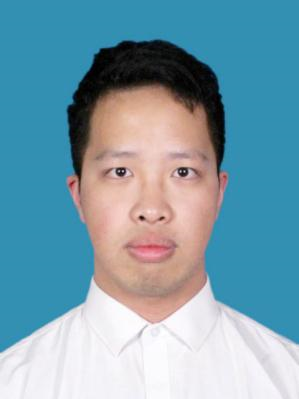
\includegraphics[width=1 in]{fig/wzx} 
%\end{figure}
%
%\noindent{\it ZiXuan Wang} was born in Nanjing, Jiangsu, China ,in 1994 . He obtained a bachelor's degree from Tongda College of Nanjing University of Posts and Telecommunications in 2017, He is currently pursuing a master's degree in logistics engineering at Nanjing University of Posts and Telecommunications, under the direction of Professor Wang. His research interests include encrypted traffic identification and data balancing.(email:wangzx@runtrend.com.cn)
%
%
%
%\begin{figure}[ht!]
%	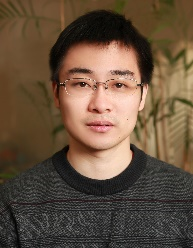
\includegraphics[width=1 in]{fig/zxk} 
%\end{figure}
%\noindent{\it Xiaokang Zhou} (M’12) received the Ph.D. degree in human sciences from Waseda University, Japan, in 2014. From 2012 to 2015, he was a research associate with the Department of Human Informatics and Cognitive Sciences, Faculty of Human Sciences, Waseda University, Japan. From 2016, he has been a lecturer with the Faculty of Data Science, Shiga University, Japan. He also works as a visiting researcher in the RIKEN Center for Advanced Intelligence Project (AIP), RIKEN, Japan, from 2017. Dr. Zhou has been engaged in interdisciplinary research works in the fields of computer science and engineering, information systems, and social and human informatics. His recent research interests include ubiquitous and social computing, big data mining and analytics, machine learning, behavior and cognitive informatics, cyber-physical-social-system, cyber intelligence and cyber-enabled applications. Dr. Zhou is a member of the IEEE CS, and ACM, USA, IPSJ, Japan, and JSAI, Japan.
%
%\begin{figure}[ht!]
%	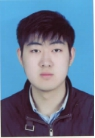
\includegraphics[width=1 in]{fig/zmx} 
%\end{figure}
%\noindent{\it Moxuan Zhang} was born on April 7, 1998. In Zhenjiang, Jiangsu Province, China. In June 2016,Graduated from High School Affiliated To Nanjing Normal University. Studied at Jinling Institute of Technology, majoring in software engineering from September 2016. (Email: zhangmoxuan\_7@126.com)

\begin{IEEEbiography}[{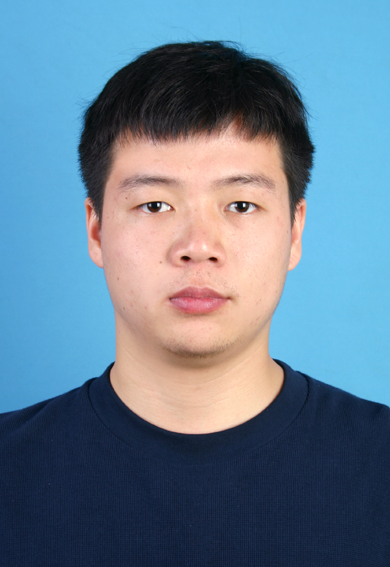
\includegraphics[width=1in,height=1.25in,clip,keepaspectratio]{fig/li}}]{ShuHang Li}

 was graduated from Jiangsu University of Science and Technology,Zhenjiang ,China, in 2013.He is currently pursuing a master's degree at Nanjing University of Posts \& Telecommunications,Nanjing China,under the direction of Professor Wang. His research direction is encrypted traffic identification,and he also interested in Deep Packet Inspection and applications.(email:lish@runtrend.com.cn)

\end{IEEEbiography}
\vspace{-30ex}
\begin{IEEEbiography}[{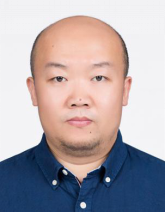
\includegraphics[width=1in,height=1.25in,clip,keepaspectratio]{fig/wp}}]{Pan Wang}
(M'18) received the BS degree from the Department of Communication Engineering, Nanjing University of Posts \& Telecommunications, Nanjing, China, in 2001, and the PhD degree in Electrical \& Computer Engineering from Nanjing University of Posts \& Telecommunications, Nanjing, China, in 2013. He is currently an Associate Professor in the School of Modern Posts, Nanjing University of Posts \& Telecommunications, Nanjing, China. His research interests include cyber security and communication network security, network measurements, Quality of Service, Deep Packet Inspection, SDN, big data analytics and applications. From 2017 to 2018, he was a visiting scholar of University of Dayton (UD) in the Department of Electrical and Computer Engineering.(email:wangpan@njupt.edu.cn)

\end{IEEEbiography}

%\vspace{-30ex}
\begin{IEEEbiography}[{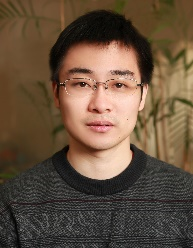
\includegraphics[width=1in,height=1.25in,clip,keepaspectratio]{fig/zxk}}]{Xiaokang Zhou}
(M’12) received the Ph.D. degree in human sciences from Waseda University, Japan, in 2014. From 2012 to 2015, he was a research associate with the Department of Human Informatics and Cognitive Sciences, Faculty of Human Sciences, Waseda University, Japan. From 2016, he has been a lecturer with the Faculty of Data Science, Shiga University, Japan. He also works as a visiting researcher in the RIKEN Center for Advanced Intelligence Project (AIP), RIKEN, Japan, from 2017. Dr. Zhou has been engaged in interdisciplinary research works in the fields of computer science and engineering, information systems, and social and human informatics. His recent research interests include ubiquitous and social computing, big data mining and analytics, machine learning, behavior and cognitive informatics, cyber-physical-social-system, cyber intelligence and cyber-enabled applications. Dr. Zhou is a member of the IEEE CS, and ACM, USA, IPSJ, Japan, and JSAI, Japan.

\end{IEEEbiography}

\vspace{-30ex}
\begin{IEEEbiography}[{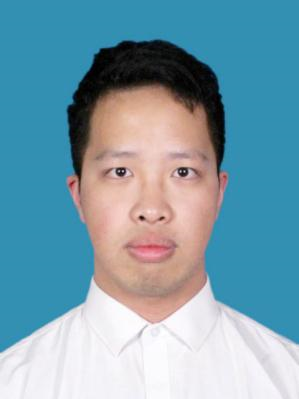
\includegraphics[width=1in,height=1.25in,clip,keepaspectratio]{fig/wzx}}]{ZiXuan Wang}
was born in Nanjing, Jiangsu, China ,in 1994 . He obtained a bachelor's degree from Tongda College of Nanjing University of Posts and Telecommunications in 2017, He is currently pursuing a master's degree in logistics engineering at Nanjing University of Posts and Telecommunications, under the direction of Professor Wang. His research interests include encrypted traffic identification and data balancing.(email:wangzx@runtrend.com.cn)

\end{IEEEbiography}

\vspace{-30ex}
\begin{IEEEbiography}[{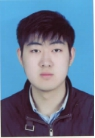
\includegraphics[width=1in,height=1.25in,clip,keepaspectratio]{fig/zmx}}]{Moxuan Zhang}
was born on April 7, 1998. In Zhenjiang, Jiangsu Province, China. In June 2016,Graduated from High School Affiliated To Nanjing Normal University. Studied at Jinling Institute of Technology, majoring in software engineering from September 2016. (Email: zhangmoxuan\_7@126.com)

\end{IEEEbiography}

\end{document}







